In the suggestion phase, we addressed the second sub-research question:
\begin{center}
    \rqTwo
\end{center}

The proposed system architecture is designed to generate recommendations regarding potential research collaborators for research projects.
Based on the literature requirements (Sec.~\ref{sec:literature-requirements}) and the application requirements (Sec.~\ref{sec:application-requirements}) derived in the problem awareness phase, the defined architecture and the approach we use allow us to fulfil these requirements.
Table~\ref{tab:requirements-fulfillment} shows the list of literature and application requirements and their corresponding fulfillment description.
The fulfilment explanation of each requirement is given later in the description of the proposed architecture.

\begin{table}[htbp]
    \centering
    \scriptsize
    \begin{tabularx}{\textwidth}{|>{\centering\arraybackslash}p{3.5cm}|X|}
      \hline
      \textbf{Literature/Application Requirement} & \textbf{Fulfillment Description}\\
        \hline
        \gls{lr}1 & The \gls{eurio} ontology encodes and provides structured, machine-readable data on EU-funded research projects\\
        \gls{lr}2 &  Similarity search and cosine similarity used as \gls{cbf} recommendation\\
        \gls{lr}3 & \glspl{kg} and \glspl{llm} integration in a \gls{rag} pipeline, combining Graph\gls{rag} and Agentic\gls{rag} to recommend research collaborators without re-training \\
        \gls{lr}4 &  Tool use and multi-agent collaboration patterns used to get retrieval of information and generate recommendations\\
        \gls{appr}1, \gls{appr}2 &  \gls{eurio} \gls{kg} provides a structured and semantically rich representation of EU-funded research projects \\
        \gls{appr}3 & Search web tool used to enrich missing information within the \gls{eurio} \gls{kg}, such as a researcher's areas of interest\\
        \gls{appr}4, \gls{appr}6 &  \gls{eurio} \gls{kg} provides a structured and semantically rich representation of EU organisations \\
        \gls{appr}5, \gls{appr}7 &  \gls{eurio} \gls{kg} provides a structured and semantically rich representation of EU participants \\
        \hline
    \end{tabularx}
    \caption{List of Literature and Application Requirements and their corresponding fulfillment description}
    \label{tab:requirements-fulfillment}
\end{table}


The proposed architecture integrates \glspl{kg} and \glspl{llm} in a \gls{rag} pipeline, following and combining the Graph\gls{rag} and Agentic\gls{rag} paradigms together.
This facilitates the recommendation of potential research collaborators without re-training the model (satisfied \gls{lr}3).
The architecture is built upon the \gls{eurio} \gls{kg}, which provides a structured and semantically rich representation of (EU-funded) research projects (satisfied \gls{appr}1, \gls{appr}2), organizations (satisfied \gls{appr}4, \gls{appr}6), and participants (satisfied \gls{appr}5, \gls{appr}7).
The \gls{eurio} ontology, as described in Sec.~\ref{sec:ontology-selection}, was found as a data model that conceptualizes, formally encodes, and makes available in an open, structured, and machine-readable format data about research projects funded by the EU's framework programmes for research and innovation (satisfied \gls{lr}1).
As shown in Fig.~\ref{fig:proposed-system-graphRAG}, the architecture consists of three main components: the Retrieval Component (red box), the Augmentation Component (purple box), and the Generation Component (blue box).
Before describing each component, we provide a brief overview of the system's user interface, the graph database, the embedding model and vector database, used in the architecture.

\begin{figure}[htbp]
    \centering
 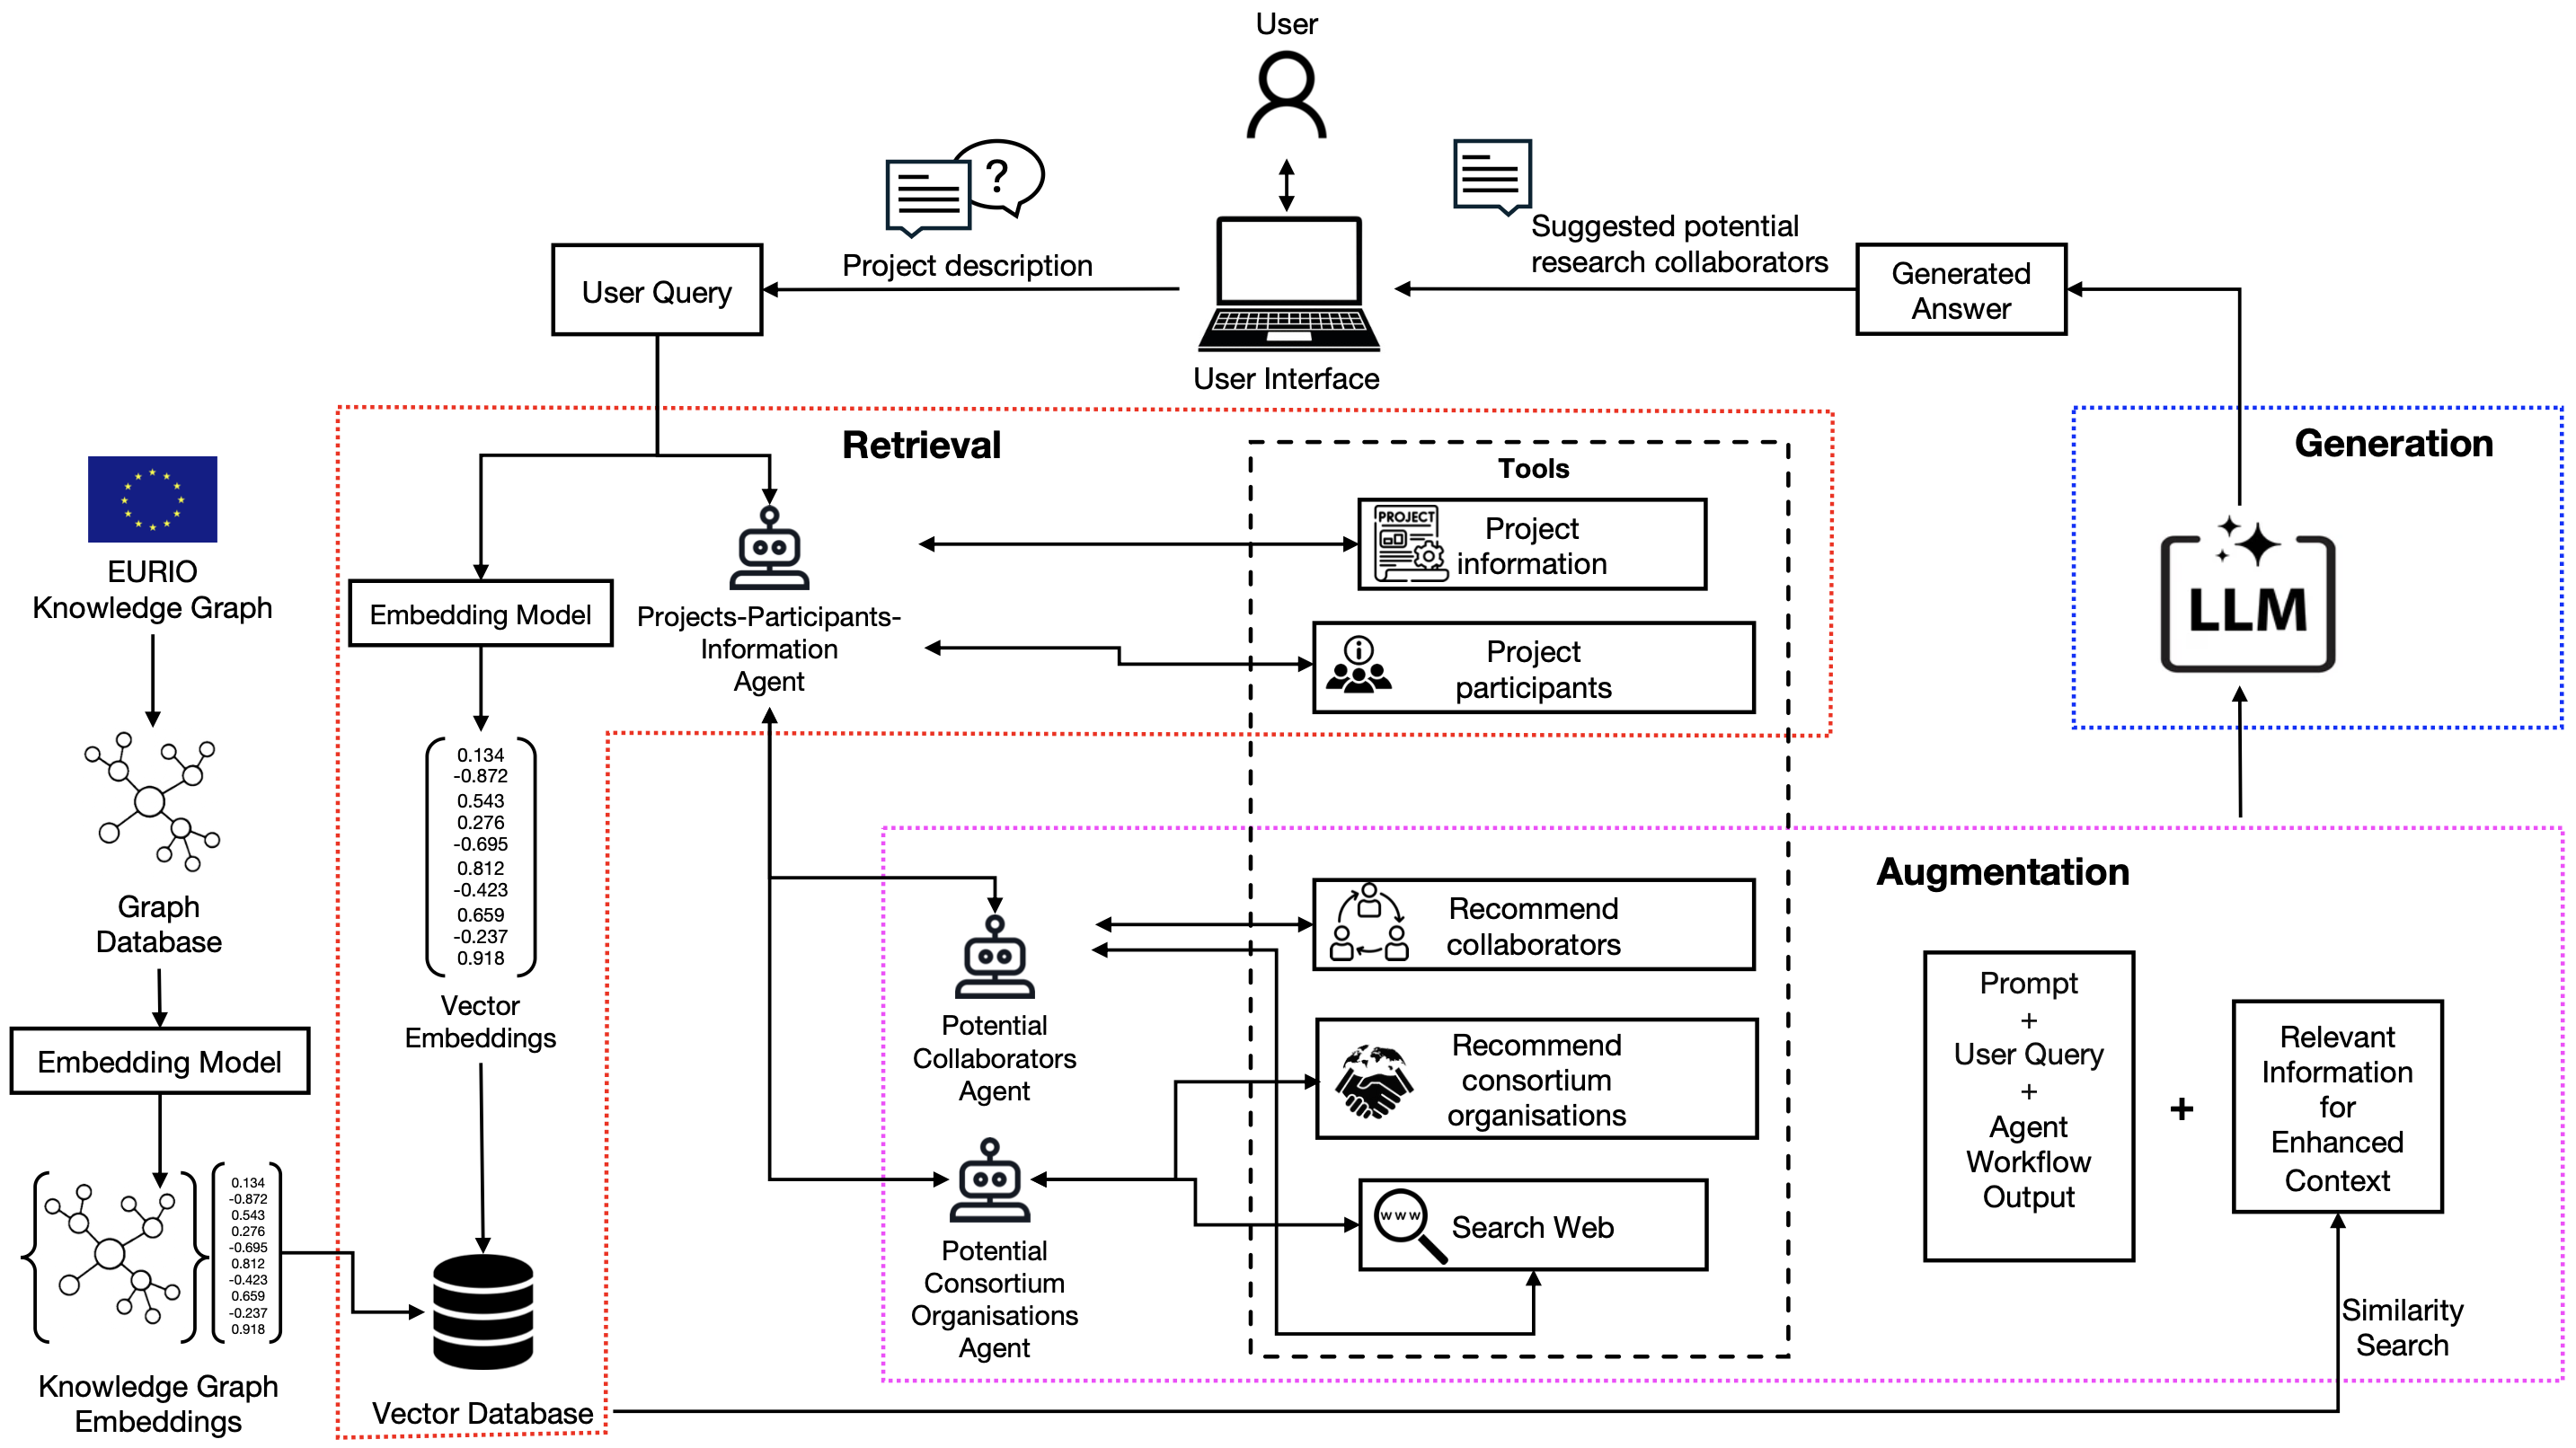
\includegraphics[width=.9\textwidth]{figures/architecture/proposed-system-graphRAG.png}
     \rule{35em}{0.5pt}
    \caption{The proposed Knowledge-Driven and Hybrid AI Architecture for Research Collaboration}
 \label{fig:proposed-system-graphRAG}
\end{figure}

\subsection*{User Interface}
The user interface of the system is designed as a chatbot to provide a user-friendly experience for researchers.
The chatbot provides information retrieval and the two types of recommendations illustrated in Sec.~\ref{sec:recommendation-strategy}.
The user can request information on people, projects and organisation details etc. in the context of European research projects.
It allows users to input a project description and objectives, and receive recommendations for potential research collaborators and consortia.
The interface is designed to be intuitive and easy to use, with clear instructions and guidance on how to input the required information.
The recommendations are displayed in a clear and structured format, with detailed information about each recommended collaborator or consortium, including their expertise, experience, and relevance to the project.

\subsection*{Graph Database}
The \gls{eurio} \gls{kg} is stored as \gls{rdf} format in a graph database, which provides a flexible and efficient way to represent and query the complex relationships between entities in the system.
The graph database allows for the storage of structured data about research projects, organizations, and participants, and enables the retrieval of relevant information based on the relationships between these entities.

\subsection*{Embedding Model and Vector Database}
The embedding model and the vector database play a crucial role in the retrieval process of the proposed system.
\gls{eurio}'s \gls{kg}, stored in a graph database, is transformed through an embedding model, which converts structured information into numerical vector representations.
These embeddings capture the semantic relationships between entities in the \gls{kg}, enabling efficient similarity searches.
The generated vector embeddings are stored in a vector database, facilitating rapid retrieval of relevant knowledge.
When a user submits a query, it is also converted into an embedding and compared against the stored vectors in a similarity search to identify relevant projects, participants, or research entities (satisfied \gls{lr}2).

\subsection*{Agentic Graph Retrieval-Augmented Generation}
Our approach combines the Graph\gls{rag} and Agentic\gls{rag} paradigms to create a hybrid \gls{ai} architecture that leverages the structured data in the \gls{eurio} \gls{kg} and the vector database to generate contextually accurate and consistent recommendations.
According to \cite{singh2025}, modern agents, such as \gls{llm}-powered and mobile agents, are intelligent entities that can perceive their environment, reason about it, and autonomously perform tasks.
In our architecture, 3 agents were defined: the \textit{Project-Participants-Information Agent}, the \textit{Project-Organization-Information Agent}, and the \textit{Project-Researcher-Information Agent}.
These agents follow two agentic workflow patterns \cite{singh2025}: the tool use pattern and the multi-agent collaboration pattern (satisfied \gls{lr}4).
As explained in the following paragraphs, the proposed architecture consists of three main components: Retrieval, Augmentation, and Generation, and agents work together within these components, using external tools to expand their capabilities to achieve specific goals.
A detailed description of each agent using its own tools is given in Sec~\ref{sec:building-ai-agents}.

\paragraph*{Retrieval Component.}
This component is responsible for retrieving relevant information from the \gls{eurio} \gls{kg} and the vector database.
The agent workflow is always initiated by the master agent: the \textit{Project-Participants-Information Agent}.
This agent is responsible for returning information about projects, such as the (e.g. project abstract), and also for returning information about the participants involved in that project (e.g. person full name, organization details).
To perform the retrieval of this information, the agent was specified to follow a template prompt, in which it is instructed to generate \gls{sparql} queries to query the \gls{eurio} \gls{kg} from which to extract data.
Depending on the task to be performed, the master agent will delegate that task to the agent responsible for that task, if necessary.

\paragraph*{Augmentation Component.}
In addition to combining the user query, prompt templates, and information retrieved from the agent master, with all relevant information obtained from the similarity search (satisfied \gls{lr}2), this component adds additional data from the activity performed by the agent workflow.
Cosine similarity was used as a metric for semantic search to determine the similarity of embeddings.
In this component, the agents \textit{Potential Collaborators Agent} and \textit{Potential Consortium Organisations Agent} are responsible for creating the recommendations.
The \textit{Potential Collaborators Agent} has the task of recommending research collaborators, given a project description as input.
The \textit{Potential Consortium Organisations Agent} has the task of creating several consortia formed by various organisations, which contribute to the consortium in a complementary way, i.e. there will be no consortia with organisations specialising in the same research area.
These two agents use the \textit{recommend collaborators} tool, and the \textit{Recommend consortium organisations} tool, respectively, to accomplish the tasks previously described, and they too are instructed with specific prompt templates to follow to achieve their goal.
In addition, both use the \textit{search web} tool, to enrich the information obtained, such as a researcher's areas of interest (satisfied \gls{appr}3), which are not present within the \gls{eurio} \gls{kg}.
In this way, agents act autonomously and are able to make dynamic decisions, resulting in better results than a graph.

\paragraph*{Generation Component.}
Finally, the generation component combines all previously retrieved and augmented information with the pre-trained knowledge of the \gls{llm} to generate contextually accurate and consistent responses.
In addition to providing relevant recommendations, this component ensures explainability by offering detailed justifications for suggested research collaborators, outlining the reasons behind their selection based on expertise, involvement in previous projects and research alignment.
It also describes how the proposed research consortia are composed, specifying the complementary roles of the participating organisations and their collective ability to achieve the project objectives.
This increases transparency and trust in the recommendation process, making the system a valuable tool for making informed decisions in research collaborations.